To "warm up" to the solving of complicated boundary value problems, we
start with a simple 1D heat diffusion problem. Consider a 1-D block of
radioactive material that produces heat at a rate $\varepsilon$,
measured in Joules per meter. In 3D this would be in J/m$^3$, but
since we reduce the problem to 1D, it is just per meter. The heat
diffusion coefficient is $D$. The temperature at the edges at $x=\pm L$
is kept fixed at $T_0$. The steady-state temperature profile obeys
\begin{equation}
    -D\cdot\frac{\partial^2T(x)}{\partial x^2}=\varepsilon
    \label{eq:temp_diffusion_equation}
\end{equation}
For simplicity let us set $D=0.5$, $\varepsilon=1$, $T_0=1$ and $L=1$.
We use $N=100$ grid points.

\paragraph{
    a) Write down the numeric form of this equation on the grid.
} \ \\
    \\
    The interval L is dicretized into $N$ equidistant points
    $(x_i)_{i \in \{1, \dots N\}}$ with
    $\Delta x = x_{i+1}-x_i = \frac{2L}{N}$. Therefore $T(x)$
    becomes $T(x_i)$, with the boundary conditions
    $T(x_1)=T(x_N)=1$. For the second derivative we use the
    three-point stencil, which yields
    \begin{align}
        -D\cdot\frac{T(x_{i+1}) - 2 T(x_i) + T(x_{i-1})}
        {(\Delta x)^2}&=\varepsilon \qquad \text{ for }i=2,
        \dots, N-1.
    \end{align}

\paragraph{
    b) Write this in matrix notation.
} \ \\
    \\
    To get the matrix notation, we interpret $T(x_i)$ as the
    $i$-th component of a vector $\vec{T}$. \\
    \\
    Then, the equations above can be expressed as
    \begin{equation}
        -\frac{D}{(\Delta x)^2} \cdot
        \begin{pmatrix}
            1     & 0     &        &\cdots &       & 0 \\
            1     &-2     & 1      & 0     &       &   \\
            0     & 1     & -2     & 1     &       &\vdots \\
            \vdots&       &\ddots  &\ddots & \ddots&  0\\
            &       &        &    1  &  -2   & 1 \\
            0     & \dots &        &      &   0   &1    \\
        \end{pmatrix}
        \begin{pmatrix}
            T(x_1) \\
            T(x_2)\\
            \vdots \\
            \\
            T(x_{N-1})\\
            T(x_N) \\
        \end{pmatrix}=\begin{pmatrix}
            -T_0D/(\Delta x)^2 \\
            \epsilon \\
            \vdots \\
            \\
            \epsilon \\
            -T_0D/(\Delta x)^2
        \end{pmatrix}
    \end{equation}
    %To avoid cancelation, we pull the - into the matrix and multiply $ \frac{(\Delta x)^2}{D} = \frac{4 L^2}{D N^2}$. The first and the last row are boundary conditions,therefore we can remove this to get regular matrix. We have to update the second and the (N-1)th equation while adding $T(x_1), T(x_N) = T_0$. Together we get
    %\begin{equation}
    %%\underbrace{
    %\begin{pmatrix}
    %2    & -1    & 0      & \dots  & 0   \\
    %-1   & 2     & -1     &        &\vdots \\
    %0    &\ddots & \ddots & \ddots &  0\\
    %\vdots&      &    -1  &    2   & -1\\
    %0    & \dots &0       &    -1  &  2 \\
    %\end{pmatrix} %}_{M}
    %%\underbrace{
    % \begin{pmatrix}
    % T(x_2)\\
    % \vdots \\
    % \\ \\ \\
    % T(x_{N-1})\\
    % \end{pmatrix} %}_{\vec{T}}
    % = \frac{4L^2 \epsilon}{D N^2}
    % \begin{pmatrix}
    % 1 \\
    % \vdots \\ \\ \\ \\
    % 1 \\
    % \end{pmatrix}
    % + \begin{pmatrix}
    % T_0 \\
    % 0\\ \vdots \\ \\ 0\\
    % T_0
    % \end{pmatrix}
    % \end{equation}

\paragraph{
    c) Now let us think of how to put this into a computer program. The
    matrix is sparse: most of the elements are zero. In fact, it is a
    special kind of sparse matrix: a tridiagonal matrix. Come up with a
    way to store the matrix elements of this tridiagonal matrix into
    only three 1D arrays of $N$ elements.
} \ \\
    \\
    A general tridiagonal matrix
    \begin{equation}
        M=
        \begin{pmatrix}
            a_1 & b_1 & 0      & 0       & 0 \\
            c_1 & a_2 & b_2    & 0       & 0 \\
            0   & c_2 & \ddots & \ddots  & 0 \\
            0   & 0   & \ddots & \ddots  & b_{n-1} \\
            0   & 0   & 0      & c_{n-1} & a_n
        \end{pmatrix}
    \end{equation} \ \\
    can be stored in three separate arrays $A$ (with length $n$) as well as
    $B$ and $C$, each with length $n-1$ as demonstrated below:
    \begin{align}
        A&=[a_1,\ a_2,\ ...,\ a_n] \\
        B&=[b_1,\ b_2,\ ...,\ b_{n-1}] \\
        C&=[c_1,\ c_2,\ ...,\ c_{n-1}]
    \end{align}

\newpage
\paragraph{
    d) Design a function/subroutine that multiplies such a matrix with
    any given vector. Test that it performs the multiplication correctly.
} \ \\
    \\
    If we are multiplying the $M$ with a vector
    $v = (v_1, \dots, v_n)^T$ we will calculate
    \begin{align}
        \begin{pmatrix}
            a_1 & b_1 & 0      & 0       & 0 \\
            c_1 & a_2 & b_2    & 0       & 0 \\
            0   & c_{i-1} & a_i & b_i    &0    \\
            0   & 0   & 0      & c_{n-1} & a_n
        \end{pmatrix}
        \begin{pmatrix}
            v_1 \\ v_2 \\v_i \\ v_n\\
        \end{pmatrix}=\begin{pmatrix}
            a_1 v_1 + b_1 v_2 \\
            c_1 v_1 + a_2 v_2 + b_2 v_3 \\
            c_{i-1} v_{i-1} + a_i v_i + b_i v_{i+1} \\
            c_{n-1} v_{n-1} + a_n v_n\\
        \end{pmatrix}
    \end{align}
    We see that the indices are sometimes shifted. To do this
    python using numpy multiplcation $\circ$ (each component), we
    define $\check{v} = (v_n, v_1, \dots, v_{n-1})^T$ and
    $\hat{v} = (v_2, v_3, \dots, v_n , v_1)^T$. With this we
    can rewrite the multiplication as
    \begin{equation}
    	Mv =
    	\begin{pmatrix} 0 \\ C \\	\end{pmatrix}
    	\circ \check{v} + A \circ v +
    	\begin{pmatrix} B \\ 0	\end{pmatrix} \circ \hat{v}
    \end{equation}
    We've tested this with $n=4$, $a_i = 2$, $b_i = -5$,
    $c_i = -1$ $ \forall i$ and $v = (0,1,2,3)^T$. The code returns
    \begin{equation}
    	Mv = (-5, -8, -12, 4)
    \end{equation}
    which is what one would expect. The python code is shown below:
    \lstinputlisting[firstline=4, lastline=5]{../code/tridiag_matrix_mult.py}
	We tested it with the
	\lstinputlisting[firstline=11,lastline=14]{../code/tridiag_matrix_mult.py}
	and got the same result as mathematica.
\newpage
\paragraph{
    e) Design and test a function/subroutine that uses the
    forward-elimination backward-substition method to solve a matrix
    equation.
} \ \\
    \\
    We do forward elimination for the eqation $Mx = r$.  $R_i$ is the i-th row,
    $\tilde{a}_i = a_i - \frac{c_{i-1} b_{i-1}}{\tilde{a}_{i-1}}$,
    $\tilde{a}_1 = a_1$,
    $\tilde{r}_i = r_i - \frac{\tilde{r}_{i-1} c_{i-1}}{\tilde{a}_{i-1}}$ and
    $\tilde{r}_1 = r_1$
    \begin{align}
	\begin{pmatrix}
	a_1 & b_1 & 0      & 0       & 0   & r_1\\
	c_1 & a_2 & b_2    & 0       & 0 & r_2\\
	0   & c_2 & \ddots & \ddots  & 0 & \vdots\\
	0   & 0   & \ddots & \ddots  & b_{n-1} &\\
	0   & 0   & 0      & c_{n-1} & a_n& r_n
	\end{pmatrix}
	\overset{R_2 = R_2 - c_1/a_1 R_1}{\sim}
	\begin{pmatrix}
	a_1 & b_1 & 0      & 0       & 0   & r_1\\
	0 & \tilde{a}_2 & b_2    & 0       & 0 & \tilde{r}_2\\
	0   & c_2 & \ddots & \ddots  & 0 & \vdots\\
	0   & 0   & \ddots & \ddots  & b_{n-1} &\\
	0   & 0   & 0      & c_{n-1} & a_n& r_n
	\end{pmatrix}
	\dots
	\begin{pmatrix}
	a_1 & b_1 & 0      & 0       & 0   & r_1\\
	0 & \tilde{a}_2 & b_2    & 0       & 0 & \tilde{r}_2\\
	0   & 0 & \ddots & \ddots  & 0 & \vdots\\
	0   & 0   & \ddots & \ddots  & b_{n-1} &\\
	0   & 0   & 0      & 0 & \tilde{a}_n& \tilde{r}_n
	\end{pmatrix}
    \end{align}
    Now we can substitute back in to get
    $x_n = \frac{\tilde{r}_n}{\tilde{a}_n} $ and
    $x_i = \frac{\tilde{r}_{i} - b_{i} x_{i+1}}{\tilde{a}_{i}}$.

	We constructed it this way
	\lstinputlisting[firstline=4, lastline=18]{../code/febs.py}
	and tested it with
	\lstinputlisting[firstline=22, lastline=28]{../code/febs.py}
	and get again the same result as mathematica.

\paragraph{
    f) Apply it to the above problem, and plot the solution to the
    above problem.
} \ \\
    \\
    This algorithm works in our case, since $M$ is diagonally
    dominant matrix and regular.
    \begin{figure}[h!]
        \centering
        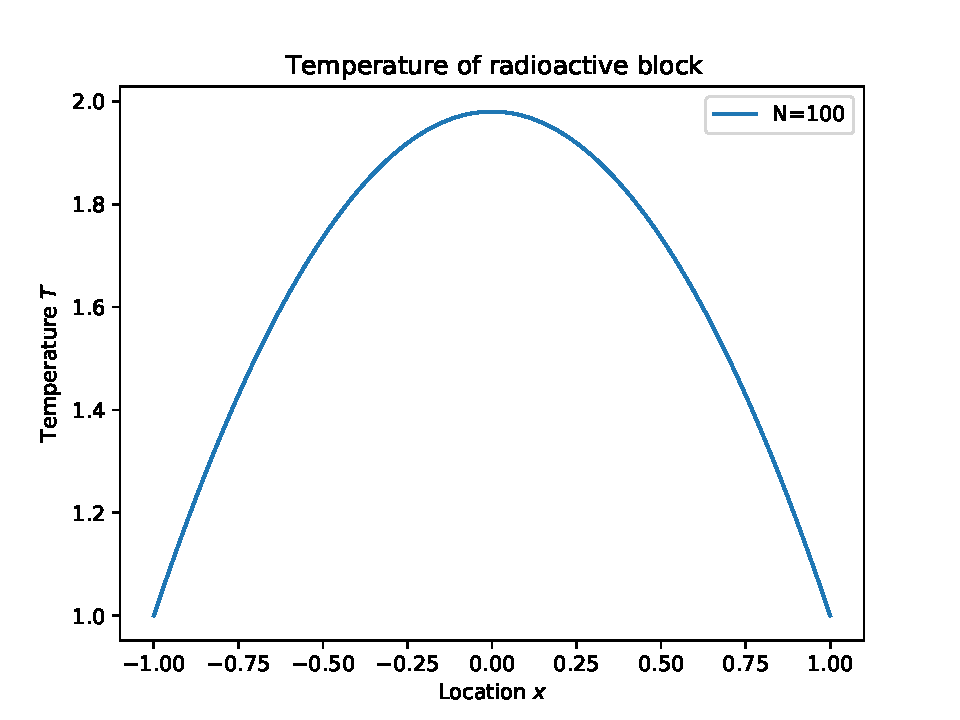
\includegraphics[width=\textwidth]{../figures/Aufg1f.pdf}
        % \caption{}
    \end{figure} \ \\

\newpage
\paragraph{
    g) Verify that the result is correct by multiplying the solution
    with the matrix and computing the residual, and show that the
    residual is almost zero.
} \ \\
    \\
    The maximum of the residuals is 5e-16. This is the order of eps.
\lstinputlisting[firstline=27, lastline=28]{../code/Aufg1.py}
\paragraph{
    h) Why is it not exactly zero?
} \ \\
    \\
numerical errors. These are arrows inorder of eps.
\paragraph{
    i) Change $N$ to e.g. 1000 and see that the result is the same, but
    smoother. As you can see, this is a very efficient method for 1D
    boundary value problems. Now let us see how the Jacobi iteration
    performs.
} \ \\
    \\
    \begin{figure}[h!]
	\centering
	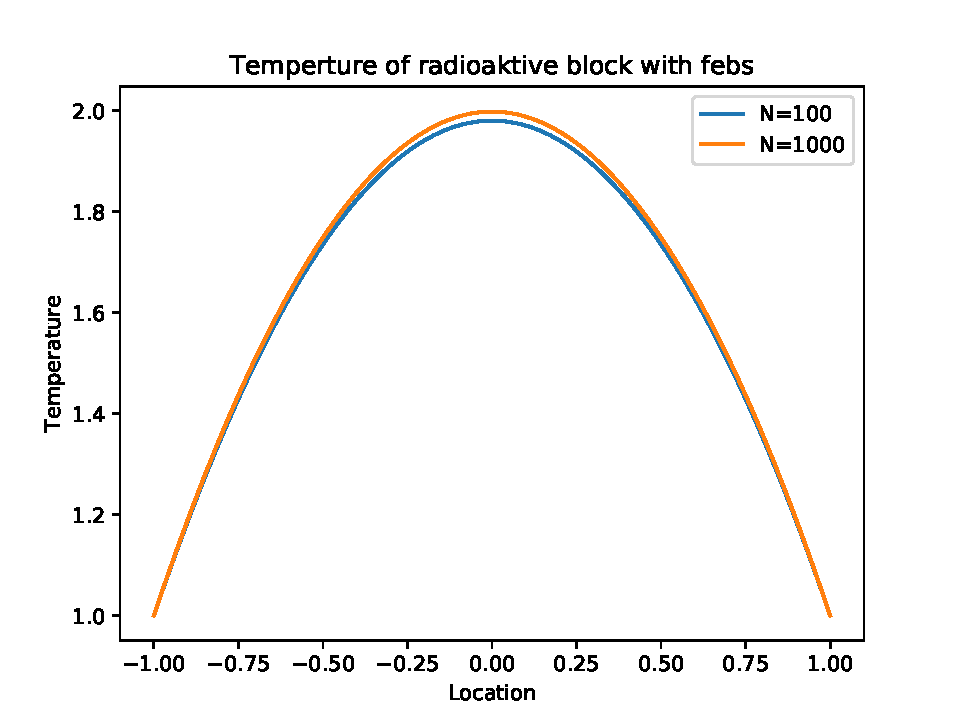
\includegraphics[width=\textwidth]{../figures/Aufg1h.pdf}
	% \caption{}
\end{figure} \ \\
\newpage
\paragraph{
    j) Design a function/subroutine to perform a single Jacobi iteration
    step for this problem. Take initially $N=8$ (yes, really that low!).
    Perform 30 iteration steps.
} \ \\
    \\

\paragraph{
    k) Plot the result of each iteration over each other, and overplot
    the true solution that we found with the forward elimination,
    backward substitution.
} \ \\
    \\
    \begin{figure}[h!]
        \centering
        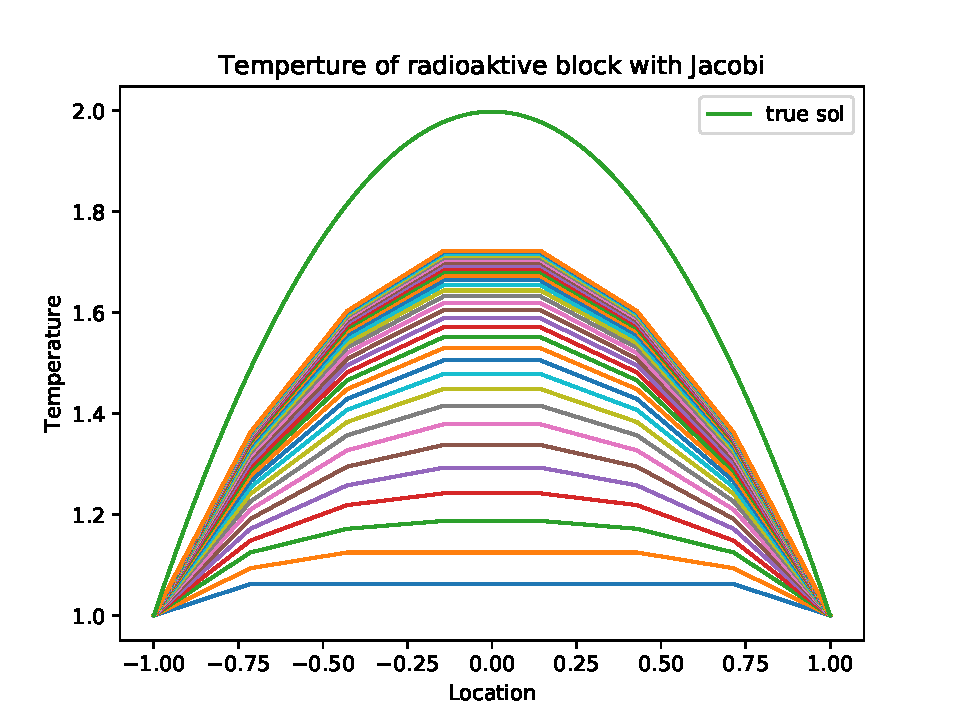
\includegraphics[width=\textwidth]{../figures/Aufg1k.pdf}
        % \caption{}
    \end{figure} \ \\

\newpage
\paragraph{
    l) Now do the same, but for $N=100$. Explain the behavior and the
    difference to the case for $N=8$.
} \ \\
    \\
    \begin{figure}[h!]
        \centering
        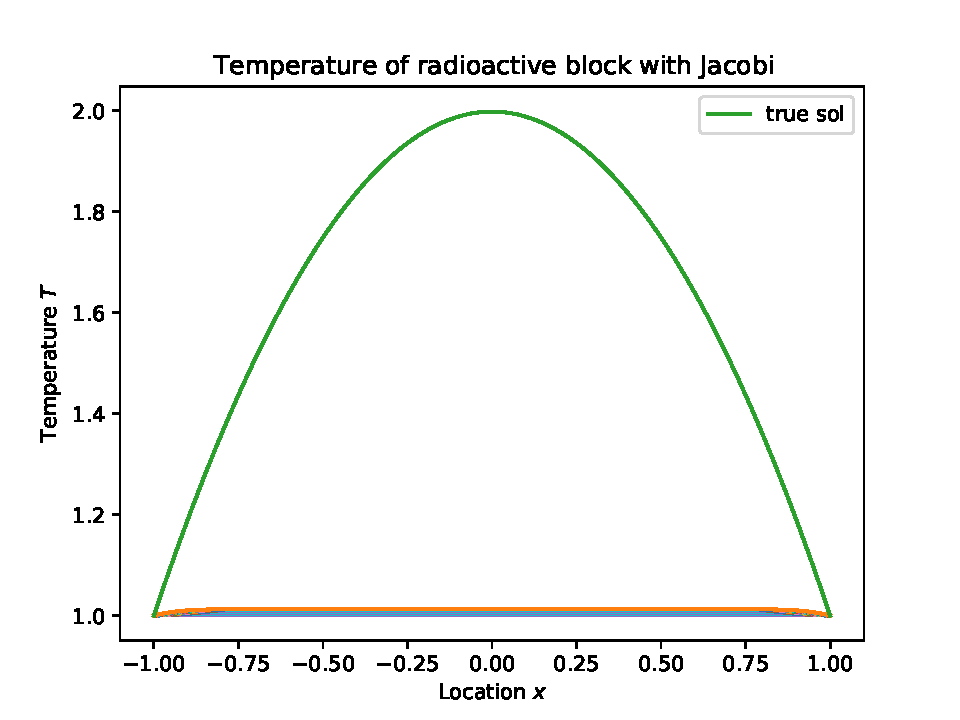
\includegraphics[width=\textwidth]{../figures/Aufg1l.pdf}
        % \caption{}
    \end{figure} \ \\

